\section{Specification of Buddy Allocation Model}
The formalization of the buddy allocation memory management consists of a model for the necessary data structures to represent the memory, and for the allocation and disposal operations memory management provides. This formalization follows the algorithms for the buddy allocation memory management in Zephyr OS, which applies a quartering split over nodes.

%This approach is more practical because it aims to pursue the efficiency. Since our specification requires a detailed description of the algorithms as well as the complex quartering way to describe, the foreseeable result is that it brings complexity to proofs than those abstract memory models.

\subsection{State Representation}
The specification begins with the structure of a quad-tree.
\begin{align*}
(set:\ 'a)\ tree = &Leaf\ (L:\ 'a)\ | \\
&Node\ (LL:\ 'a\ tree)\ (LR:\ 'a\ tree)\ (RL:\ 'a\ tree)\ (RR:\ 'a\ tree)
\end{align*}

We use recursive method to construct a quad-tree. It has two forms: \emph{Leaf} tree and \emph{Node} tree. A \emph{Node} tree is built by itself or a \emph{Leaf} tree. The notation \emph{Leaf} means the end of this construct process. Notations \emph{LL}, \emph{LR}, \emph{RL} and \emph{RR} return corresponding subtrees of the \emph{Node} tree. We use type \emph{block} to instantiate the polymorphic notation \emph{'a} in the quad-tree structure. Type \emph{block} is a record type that consists two subtypes: \emph{block\_state\_type} (indicated as \emph{ALLOC} and \emph{FREE} that constructed by \emph{datatype} function); \emph{ID} (in basic type of \emph{nat}). Notion \emph{block\_state\_type} stands for the usage state of a block and \emph{ID} represents a range of address occupied by a memory block. Notion \textbf{set} means a function that collects all records of the leaves from a quad-tree.

In addition, we create some auxiliary functions conducted on the \textsl{block tree}. Function \textbf{get\_level} (\textbf{btree::block tree}) $\Rightarrow$ (\textbf{b::block tree}) $\Rightarrow$ (\textbf{level::nat}) returns the \emph{level} where the subtree \emph{b} locates in \emph{btree} from the root whose level is 0. Function \textbf{allocsets} (\textbf{btree::block tree}) $\Rightarrow$ (\textbf{aset::block set}) returns a set of records \emph{aset} of the leaves whose \emph{block\_state\_type} is \emph{ALLOC} from the quad-tree \emph{btree}. Function \textbf{freesets} has similar definitions but returns \emph{FREE} ones. Function \textbf{freesets\_level} (\textbf{btree::block tree}) $\Rightarrow$ (\textbf{level::nat}) $\Rightarrow$ (\textbf{fset::block set}) collects all records of the leaves whose \emph{block\_state\_type} is \emph{FREE} and locate at \emph{level} in the quad-tree \emph{btree} as a set \emph{fset}. We use a notation \emph{idset} to represent the collection of all used \emph{IDs}. To create a new leaf, we have to pick up a new \emph{ID} to mark this new leaf by the strategy of \emph{SOME p. p} $\notin$ \emph{idset}.

Before introducing allocation model, we create a function \textbf{output\_level} that maps request sizes to the most suitable allocation levels in a quad-tree. The input parameters are \emph{blo\_list::nat list} and \emph{rsize::nat}. Static linked list \emph{blo\_list} is used to store the size of blocks for each level in a quad-tree and its indexes represent the levels of a quad-tree. For example, the size of root is 1024\emph{Mbytes} and the first level is 256\emph{Mbytes}, then \emph{blo\_list}!0 is equal to 1024 and \emph{blo\_list}!1 is 256. The \emph{blo\_list} is a strictly decreasing list to simulate the fact that the smaller the level, the larger size the memory block. It returns a index \emph{l} of \emph{nat} in \emph{blo\_list} with these constrains: the size it represents has to be greater than or equal to the size of request block, and there is no smaller size that meets this condition. After that, the most suitable block size is picked up from \emph{blo\_list}, and then mapped to the correct level of the quad-tree by the index \emph{l} in \emph{blo\_list}. We use \emph{rlv} to represent the output. The definition of this mapping is as follows.

\begin{definition} [Mapping Request Sizes to Allocation Levels] \\
	output\_level blo\_list rsize $\equiv$ THE l. l $<$ $\vert$blo\_list$\vert$ $\wedge$ rsize $\le$ blo\_list ! l $\wedge$ \\
	\phantom{x} \hspace{10pt} ($\vert$blo\_list$\vert$ $>$ 1 $\wedge$ l $<$ $\vert$blo\_list$\vert$ - 1) $\longrightarrow$ rsize $>$ blo\_list ! (l+1)
\end{definition}

\subsection{Allocation Model}
Based on the above structure of a quad-tree, we specify allocation operation as function \textbf{alloc}. Firstly, we introduce two assistant functions. Function \textbf{exists\_freelevel} (\textbf{bset::block tree set}) $\Rightarrow$ (\textbf{rlv::nat}) $\Rightarrow$ (\textbf{re::bool}) checks that whether there is a quad-tree in \emph{bset} (the collection of all quad-trees in memory system) that has such free leaves whose level is less than or equal to \emph{rlv}. Function \textbf{freesets\_maxlevel} (\textbf{bset::block tree set}) $\Rightarrow$ (\textbf{rlv::nat}) $\Rightarrow$ (\textbf{lmax::nat}) returns the maximum level \emph{lmax} among all levels with free leaves but less than or equal to \emph{rlv}. The definitions are as follows.

\begin{definition} [existence of free blocks in a level] \\
	exists\_freelevel bset rlv $\equiv$ $\exists$l. l $\leq$ rlv $\wedge$ $\exists$b $\in$ bset. freesets\_level b l $\ne$ $\emptyset$
\end{definition}

\begin{definition} [maximum level of free blocks] \\
	freesets\_maxlevel bset rlv $\equiv$ \\
	\phantom{x} \hspace{10pt} THE lmax. lmax $\leq$ rlv $\wedge$ \\
	\phantom{x} \hspace{60pt} $\exists$b $\in$ bset. freesets\_level b lmax $\neq$ $\emptyset$ $\wedge$ \\
	\phantom{x} \hspace{60pt} $\forall$l $\leq$ rlv. $\exists$b $\in$ bset. freesets\_level b l $\ne$ $\emptyset$ $\longrightarrow$ l $\leq$ lmax
\end{definition}

During the allocation precess, if no such leaf right in the requested level exists but bigger leaves exist, then it is necessary to split a bigger leaf into small leaves until the leaf that satisfies the request appears. Function \textbf{split} (\textbf{b::block tree}) $\Rightarrow$ (\textbf{lv::nat}) $\Rightarrow$ (\textbf{btree::block tree}) divides an original leaf \emph{b} into a subtree \emph{btree} by recursion for \emph{lv} times. The division operation always conducts on the leftmost subtree. A simple example describing this process is showed in Fig. \ref{fig1} until free leaf in the request level appears and then be allocated.

\begin{figure}
	\centering
	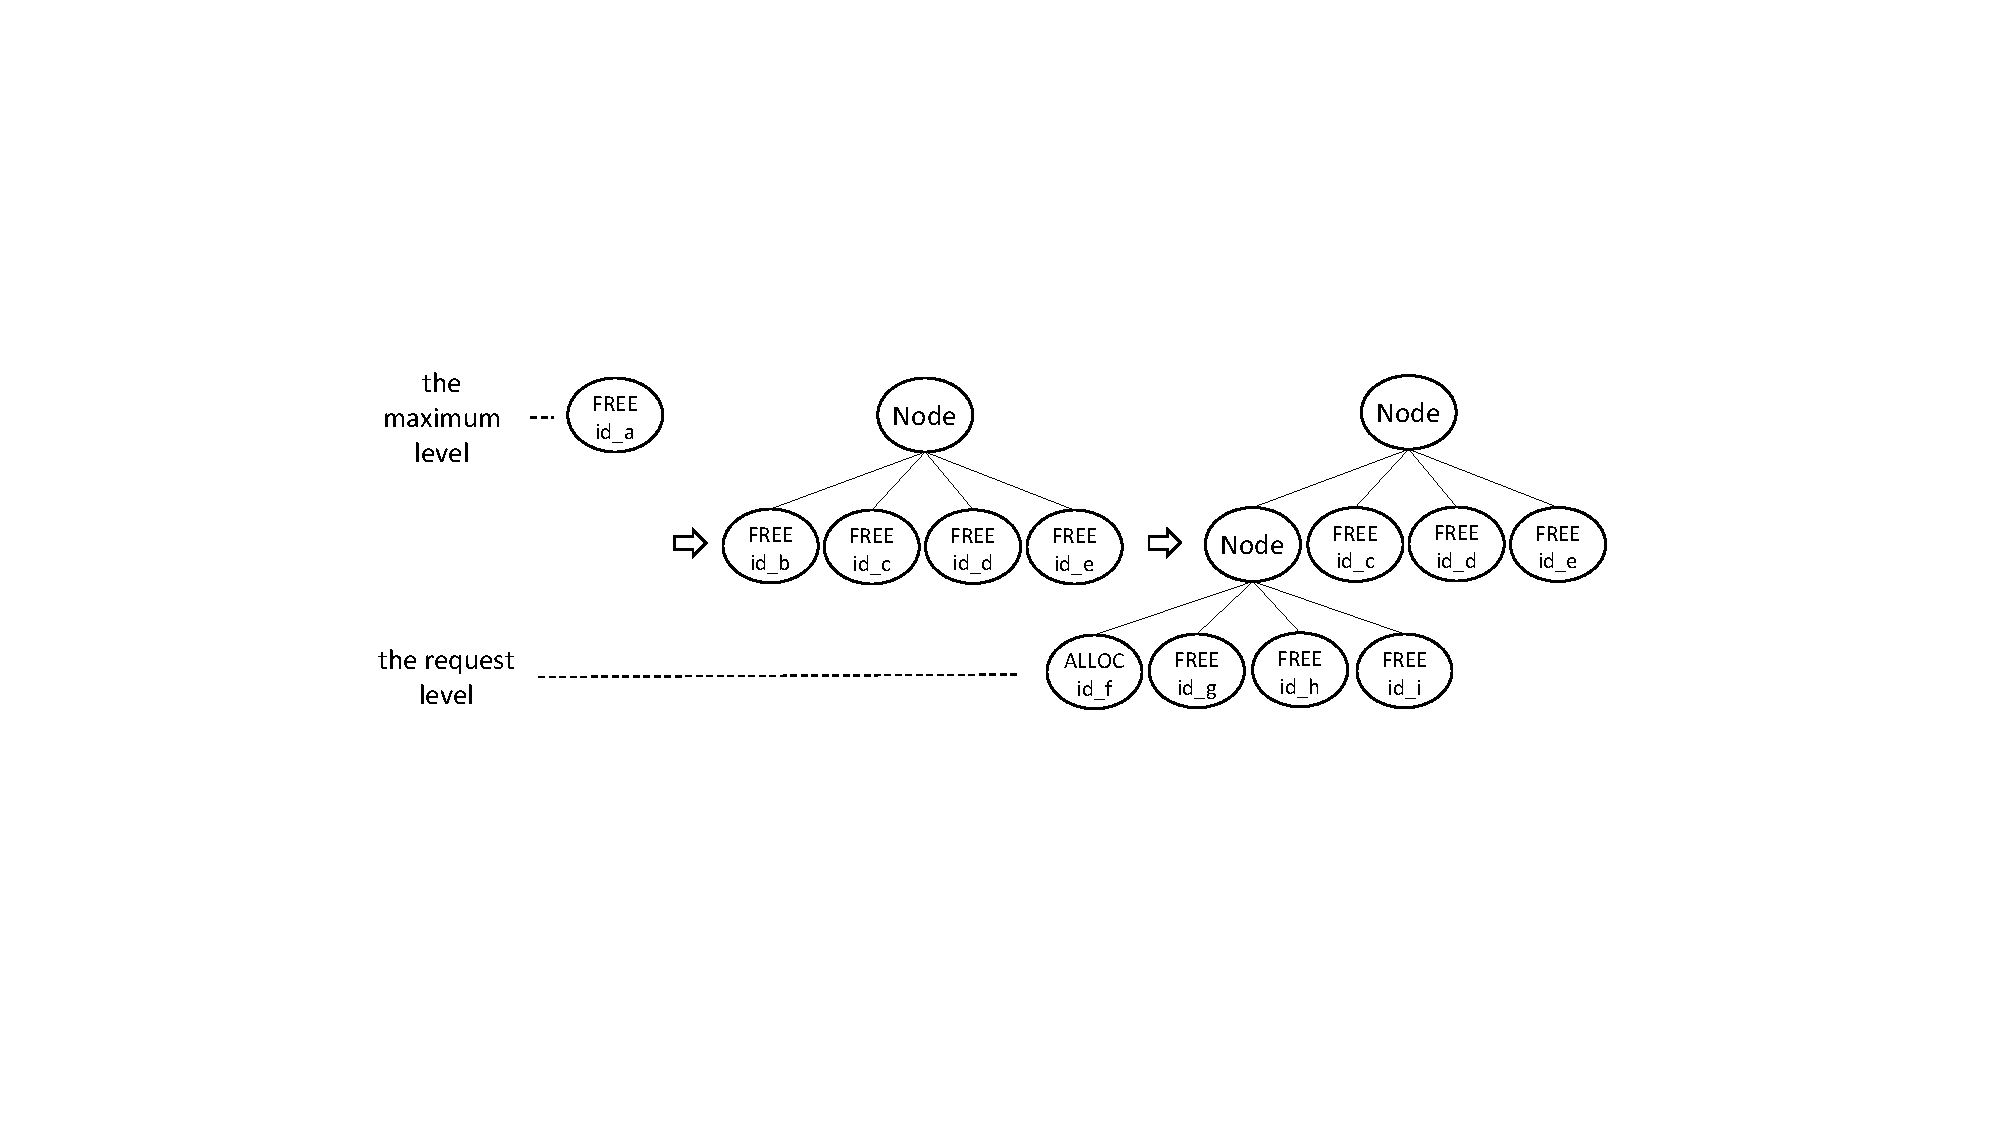
\includegraphics[width=1\textwidth]{fig1.pdf}
	\caption{The progress of dividing a free leaf}
	\label{fig1}
\end{figure}

We define the \emph{split} operation as follows. 
Function divide takes a Leaf node $b$ and returns a new non-terminal Node $n$ with four terminal Leaf nodes. The leftmost Leaf of $n$ is marked as allocated, while the rest subnodes are marked as free.

Among its definition, function \textbf{divide} (\textbf{b::block tree}) $\Rightarrow$ (\textbf{btree::block tree}) is a small step that splits an original leaf \emph{b} into a \emph{Node} tree \emph{btree} once and sets the \emph{LL} subtree to \emph{ALLOC}.

\begin{definition} [splitting a leaf] \\
	split b lv $\equiv$ \\
	\phantom{x} \hspace{10pt} if lv = 0 then b \\
	\phantom{x} \hspace{10pt} else Node (split (LL divide b) (lv - 1)) (LR divide b) (RL divide b) (RR divide b)
\end{definition}

After all auxiliary functions have been defined, now we give the process of allocation operation. It firstly checks whether there is a quad-tree in \emph{bset} that has such free leaves whose level is less than or equal to \emph{rlv} by function \emph{exists\_freelevel}. If it returns \emph{False} then the allocation process stops and returns original \emph{bset} and \emph{False}. Otherwise, function \emph{freesets\_maxlevel} return the maximum level \emph{lmax} among all levels with free leaves but less than or equal to \emph{rlv}. If the \emph{lmax} is equal to requested level \emph{rlv}, then randomly pick up such a quad-tree as \emph{btree} and pick up such a leaf from it to allocate. 


The definition of allocation operation is as follows.

\begin{definition} [Allocation Operation] \\
	alloc bset rlv $\equiv$ \\
	\phantom{x} \hspace{10pt} if exists\_freelevel bset rlv then \\
	\phantom{x} \hspace{20pt} lmax = freesets\_maxlevel bset rlv \\
	\phantom{x} \hspace{20pt} if lmax = rlv then \\
	\phantom{x} \hspace{30pt} btree = SOME b. b $\in$ bset $\wedge$ freesets\_level b rlv $\ne$ $\emptyset$ \\
	\phantom{x} \hspace{30pt} l = SOME l. l $\in$ freesets\_level btree rlv \\
	\phantom{x} \hspace{30pt} return (bset - $\lbrace$btree$\rbrace$ $\cup$ (reset btree l ALLOC) $\times$ True) \\
	\phantom{x} \hspace{20pt} else \\
	\phantom{x} \hspace{30pt} btree = SOME b. b $\in$ bset $\wedge$ freesets\_level b lmax $\ne$ $\emptyset$ \\
	\phantom{x} \hspace{30pt} split (SOME l. l $\in$ freesets\_level btree lmax) (rlv - lmax) \\
	\phantom{x} \hspace{30pt} return (bset - $\lbrace$btree$\rbrace$ $\times$ True) \\
	\phantom{x} \hspace{10pt} else return (bset $\times$ False)
\end{definition}

\subsection{Deallocation Model}

\begin{definition} [Deallocation Operation] \\
	free blo\_set b $\equiv$ \\
	\phantom{x} \hspace{10pt} if $\exists$btree $\in$ blo\_set. b $\in$ tree.set btree then \\
	\phantom{x} \hspace{20pt} if type b = FREE then False \\
	\phantom{x} \hspace{20pt} else btree = THE t. t $\in$ blo\_set $\wedge$ b $\in$ tree.set t \\
	\phantom{x} \hspace{40pt} merge (reset btree b FREE) \\
	\phantom{x} \hspace{10pt} else False
\end{definition}

The deallocation progress firstly checks whether there is a quad-tree in \emph{blo\_set} that the occupied memory block to be released belongs to this tree. If there is no such tree, the procedure returns \emph{False}. Next, if the type of the occupied memory block is \emph{FREE}, the progress also returns \emph{False}. When all conditions are met, the memory block is returned to the tree it belongs to, thereafter merging operation is executed. The merging operation is to combine all free memory blocks that belong to the same parent tree showed in Fig. \ref{fig2}.

\begin{figure}
	\centering
	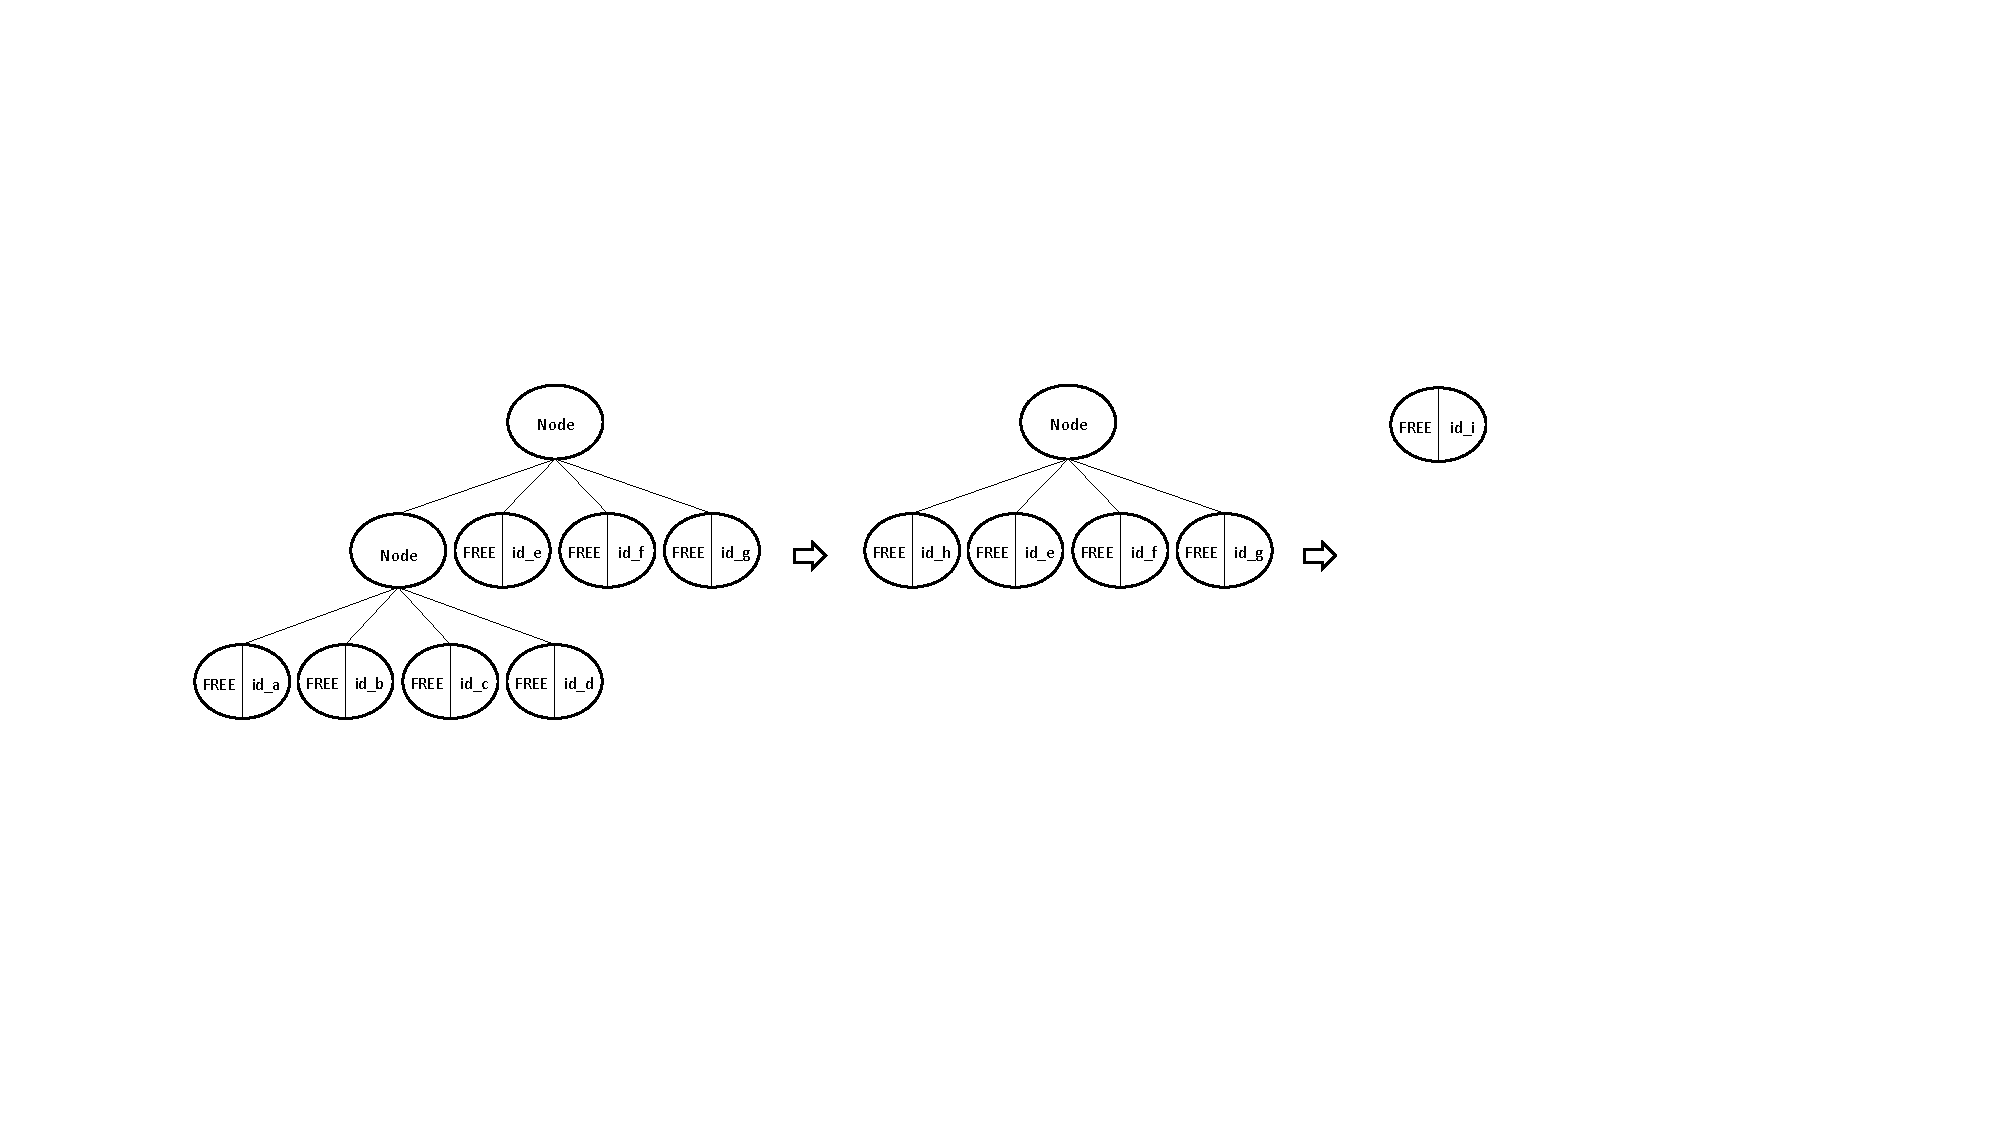
\includegraphics[width=1\textwidth]{fig2.pdf}
	\caption{The progress of merging all free memory blocks}
	\label{fig2}
\end{figure}

Owing to space constraints, the \emph{split} and the \emph{merge} operations constructed by induction are not described in detail. At this point, we have done the specification for the buddy memory algorithms. Next, we are going to verify the properties to guarantee the functional correctness of this specification.